
Elliptic curves have a rich and beautiful history, and having been studied by mathematicians for over a hundred years. They have been used to solve a diverse range of problems. For instance the congruent number problem asks for a classification of the positive integers occurring as the area of some right-angled triangle, the lengths of whose sides
are rational numbers. Another example is proving \textit{Fermat’s Last Theorem } which states
that the equation \EquationFermatLastTheorem ~ has no nonzero integer solutions for $x,y$ and $z$ when the integer $n$ is greater than $2$. 

In 1985, Neal Koblitz and Victor Miller independently proposed their solution on how to design public-key cryptographic systems using elliptic curves. During the late 1990’s elliptic curve systems started receiving commercial acceptance
when accredited standards organizations specified elliptic curve protocols and private companies started to include these protocols in their commercial products. 

However, there are usually several criterias that need to be addressed when selecting a family of public-key
schemes for such domain-specific application. In general, these security principals are \textit{functionality}, \textit{security} and \textit{performance}. The first one answers the question \textit{does the chosen public-key family provide the desired capabilities ?}, while the second principal examines the assurance protocol security. Lastly, the third principle evaluates that the primary objective are meeting the desired level of security from the performance perspective. 

In practice other factors (outside of the previous three mentioned) that may influence the decision are for instance the existence of best-practice standards (usually developed by accredited standards organizations), perhaps the availability of commercial cryptographic products, patent coverage, etc.  

Let us depict the \textit{Base Communication} model as shown in  \refFigure{fig:ch1.cryptographybasiccommunicationmodel}. Given two entities $A$ (Alice) and $B$ (Bob) who are communicating over an \textit{unsecured channel}.  Such specific scenario may be arise when for example $A$ and $B$ are communicating over a cellular telephone network, or an individual person $A$ who is in the process of purchasing a product from an online store $B$ represented by its web site $B$.  Another practical example when $A$ is sending let say an email message to $B$ over the Internet.

 In every case, $E$ could attempt to read the traffic from $A$ being send to $B$ from the unsecured channel, or modify selected portions of such message. 

\begin{figure}[h]
	\centering
	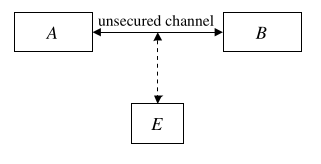
\includegraphics[width=0.5\linewidth]{98_Pictures/Chapter_01/intro_chapter/cryptography_basic_communication__model}
	\caption[Basic communication model between $A$ (Alice) and $B$ (Bob) over and unsecured channel]{\textit{Base Communication Model}. Entities $A$ (\textit{Alice}) and $B$ (\textit{Bob}) communicates over an unsecured channel. $E$ (Eve) represents the malicious entity, who is able to read, modify messages and/or impersonate entites. }
	\label{fig:ch1.cryptographybasiccommunicationmodel}
\end{figure}

Given that specific scenario we are being presented by fundamental objectives of secure communications:  Firstly, we can speak about \textit{confidentiality} with the purpose of keeping the data secret from all but authorized party members to see it, for example the messages being sent by $A$ to $B$ should not be readable by $E$.

Next, we might think about \textit{data integrity} which ensures that data has not been altered by any unauthorized means, therefore $B$ should be able to detect when data sent by $A$ has been modified by $E$. Similarly, this should yield the same result from the perspective of the other party member:  $B$ should be able to verify that data purportedly sent by $A$ indeed originated with $A$ (commonly referred as \textit{entity authentication}).

The last objective is referred as \textit{non-repudiation}, with goal to prevent an entity from denying previous commitments or actions. For instance when $B$ receives a message purportedly from $A$, not only is $B$ convinced that the message originated with $A$, but $B$ can convince a neutral  third party of this, thus $A$ cannot deny having sent the message to $B$. 

Based on the consideration how the communicating entities agree upon keyring material during their communication, cryptographic systems can be broadly divided into two kinds: symmetric-key and public-key schemes as depicted in \refFigure{fig:ch1.symmetric-vs-public-key-scheme}. With the previously demanded security objectives in mind, and given the method of use it can be a decisive factor in choosing between symmetric and public-key cryptographic systems. 

\begin{figure}[h]
	\centering
	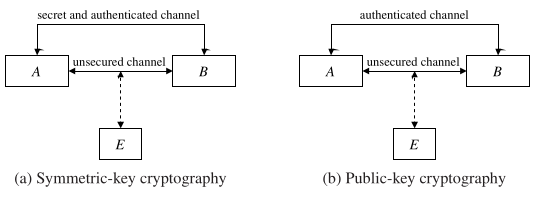
\includegraphics[width=0.7\linewidth]{98_Pictures/Chapter_01/intro_chapter/symmetric-vs-public-key-scheme}
	\caption[Comparison of Symmetric-key and Public-key Cryptography Schemes]{Comparison of Symmetric-key and Public-key Cryptography Schemes}
	\label{fig:ch1.symmetric-vs-public-key-scheme}
\end{figure}

In symmetric-key schemes (depicted in the left subfigure of \refFigure{fig:ch1.symmetric-vs-public-key-scheme}), the communicating entities first agree upon keying material that is both secret and authentic. Subsequently, they may use a symmetric-key encryption scheme such as the \textit{Advanced Encryption Standard } (AES) \cite{nist.fips197} to achieve confidentiality, in conjunction  with the use a \textit{message authentication code} (\acs{acronym.definitions.messageauthenticationcode}) algorithm such as  \acs{acronym.definitions.hmac}\cite{nist.fips198} to achieve data integrity and to preserve origin authentication. 

The major advantage of symmetric-key cryptography is it's high efficiency. However, there some significant drawbacks to these systems given our scenario. One primary drawback is the infamous \textit{key distribution problem}, with the requirement for a channel to be both secret and authenticated for the distribution of keying material is essential. On top of that in a network of $N$ entities, each entity may have to maintain different keying material with each of the other $N-1$, as commonly referred in the \textit{key management problem}. 

\subsection{Diffie-Hellman Public-Key Encryption/Decryption Scheme}
\label{ssec:ch1.diffiehellmankeyencryptionscheme}

In 1967 Diffie and Hellman showed that two parties can establish a shared secret over an insecure channel (such as depicted in  \refFigure{fig:ch1.cryptographybasiccommunicationmodel}) without any prior knowledge of one
another. Since one cannot gain any intuition towards their groundbreaking result without being aware of the existence of \textit{one-way functions}, I will primarily refer \cite{costello.fast.formulas.thesis,BF01, DH76, menezes2004ECC} in this subsection and for the following \refSubsection{sec:ch1.diffihellmannassumptionsellipticurvesecurity}.


A \textit{one-way function} is one that is easy to compute in "one direction", but which is
believed infeasible to compute from the other direction. In their paper Diffie and Hellman used the 
exponentiation in finite fields as an example to introduce the notion of public-key cryptography.  More specifically, they showed that a party member $A$ can bury their secret value $a$ by raising some publicly known generator $g$ to the power of $a$ in $\FieldF_q$:  for instance, by computing $g_a = g^a \in \FieldF_q$ . Then $A$'s public key  (denoted as $g_a$ ) can then be sent over the insecure channel to another party $B$, whose secret value is $b$, to which $B$ can exponentiate $g_a$ and compute $g_{ab} = g^a_b$ . Conversely, $b$ can compute their public key $g_b = g^b$ and send it over an insecure channel to $A$, who can compute the shared secret $gab = g^b_a$.

In contrast to symmetric-key schemes, public-key schemes (as can be followed in \refFigure{fig:ch1.symmetric-vs-public-key-scheme}) only requires the authenticity of the exchange keying material of communicating entities, but which does not have to be secret. Each entity then selects a single key pair $(e, d)$ consisting of a public key $e$, and a related private key $d$ (that the entity keeps secret). Such keys have the property that it is computationally infeasible to determine the private key solely from knowledge of the public key. 

Let say an entity $A$ wishes to send entity $B$ a confidential message noted as $m$, she she will obtain an authentic copy of $B$’s public key $e_B$. As a next step she uses the encryption function of a public-key encryption scheme to compute the ciphertext, formulated as $c = \mathsf{ENC}_{e_B}(m)$. $A$ then transmits $c$ to $B$, who uses the decryption function on his private key $d_B$ to recover the plaintext, formulated as $m= \mathsf{DEC}_{d_B}(c)$. 

In such relation it is essential only that $A$ obtain an authentic copy of $e_B$, thus confidentiality can be satisfied.  Furthermore to satisfy non-repudiation objective \textit{Digital Signature Schemes} may be devised for data origin authentication and data integrity. 
% and to facilitate the provision of non-repudiation services as can be further followed in \cite{menezes2004ECC}. 

In both  cases the individual secrets of both parties are assumed to be safe under the  \ac{acronym.algorithmcomplexity.dlp.lowerItalic} in $\FieldF_q$, which is
defined as follows: given $g \in \FieldF_q$ and $h = g^x \in \FieldF_q$, find $x$.  If $q$ is large enough, so that solving the DLP is infeasible, then the exponentiation is the \textit{one-way function} that keeps $a$ and $b$ out of reach for eavesdroppers and attackers. In addition, we assume that computing $g_{ab} = g^{ab}$ is infeasible for adversaries that know $g, g_a$ and $g_b$,  yielding us with the Diffie-Hellman problem in $\FieldF_q$. \cite{costello.fast.formulas.thesis, BF01}

\subsubsection{Discrete Logarithm Problem}
\label{ssec:ch1.dlogproblem}



The first published public-key construction by Diffie and Hellman was based on the discrete logarithm problem in the finite field \mathFormulaObject{\FieldF_p}, where $p$ denotes a (large) prime.  Using the \textit{Primitive Root Theorem}\cite{hoffsteinintrotomathematicalcryptograhpy} tells us, that given $p$  prime number, then there exists an element \FieldFpStar~ whose powers give every element of \FieldFpStar~ in the form of \refEquation{eq:ch1.primitiveroottheorem}:

\insertEquationEnvironmentWithLabel{
	\FieldFpStar = \{ 1,g, g^2, g^3, \ldots, g^{p-2} \}
}{eq:ch1.primitiveroottheorem}

%% pp. 45 from Introduction To Mathematica
The elements of \refEquation{eq:ch1.primitiveroottheorem} with this property are called the \textit{primitive roots} of \mathFormulaObject{\FieldF_{p}} or generators of \FieldFpStar, as we saw previously in \refDef{eq:ch1.multiplicativeGroup}. Such generators can be seen as the elements of \FieldFpStar~ having order of $p-1$.  This means that every nonzero element of \FieldFp~ is equal to some power of $g$.  Now, with the definition of  primitive root for \FieldFp, we can reformulate the \textit{Discrete Logarithm Problem} as follows \cite{hoffsteinintrotomathematicalcryptograhpy}.

\insertDefinitionEnvironment{
	Let $g$ be a primitive root for \FieldFp, while $h$ be a nonzero element of \FieldFp. Than the \textit{Discrete Logarithm Problem} (\acs{acronym.algorithmcomplexity.dlp}) is the problem to find an exponent of $x$ such that:
	
	\insertEquationEnvironment{
		\mathFormulaTwoSidesCongruent{g^x}{h  \left(\bmod p\right),}
	}
	
\noindent where $x$ is called the \textit{discrete logarithm of } $h$ to the base $g$ and is denoted by $\log_g(h)$.
}

% Menezes
\subsection{Security assumptions related to Elliptic Curve-based Cryptosystems }
\label{sec:ch1.diffihellmannassumptionsellipticurvesecurity}

For the sake of completeness, we must have mention the case of the discrete logarithm problem discussed in \refSubsection{ssec:ch1.dlogproblem} as it pertains to elliptic curves as well.  However, we note that there are several known formulations of the discrete logarithm problem ( refer to \cite{maya6} ), but this subsection includes only those definitions that, based on sources \cite{menezes2004ECC} and \cite{BF01}, aid in understanding the subsequent sections. 

Since the hardness of the elliptic curve discrete logarithm problem is essential for the security of all elliptic curve cryptographic schemes first we start the generalization of the discrete logarithm problem for elliptic curves.

\insertDefinitionEnvironment{
The elliptic curve discrete logarithm problem (\acs{acronym.algorithmcomplexity.ecdlp}) is as follows. Given an elliptic curve $E$ defined over a finite field $\FieldF_q$, a point $P \in E(\FieldF_q)$ of order $n$, and a point $Q \in \langle P \rangle$. The goal is to find the integer $l \in [0, n-1]$ such that $Q = lP$. Where the integer $l$ is called the discrete logarithm of $Q$ to the base $P$, denoted as $l= \log_P Q$.
\label{def:acronym.algorithmcomplexity.ecdlp}
}


While hardness of the \acs{acronym.algorithmcomplexity.ecdlp} is necessary for the security of any elliptic curve cryptographic scheme, it is generally not sufficient. As the referenced articles presents, some problems related to the \acs{acronym.algorithmcomplexity.ecdlp} whose hardness is assumed in the security proofs for some elliptic curve protocols.

\insertDefinitionEnvironment{
	The (computational) elliptic curve Diffie-Hellman problem (ECDHP  \acs{acronym.algorithmcomplexity.ecdhp}) is: given an elliptic curve $E$ defined over a finite field \mathFormulaObject{\FieldF_q}, a point $P \in E(\FieldF_q)$ of order $n$ and points $A = aP, B=bP \in \langle P \rangle$. Than the problem can be expressed as to find the point $C = abP$.
	\label{def:acronym.algorithmcomplexity.ecdhp}
}

If the ECDLP in $\langle P \rangle$ can be efficiently solved, then the ECDHP in $\langle P \rangle$ can also be efficiently solved by first finding a from $(P, A)$ and then computing $C = a B$. Thus the \acs{acronym.algorithmcomplexity.ecdhp} is no harder than the \acs{acronym.algorithmcomplexity.ecdlp}.


The elliptic curve decision Diffie-Hellman problem (\acs{acronym.algorithmcomplexity.ecddhp}) is formulated as follows:

\insertDefinitionEnvironment{
	Given an elliptic curve $E$ defined over a finite field $\FieldF_q$, a point $P \in E(\FieldF_q)$ of order $n$, and points $A=aP, B=bP, C=cP \in \langle P \rangle$. The goal is to determine wheter $C = abP$ or \mathFormulaTwoSidesCongruent{c}{ab (\bmod n) }.
	\label{def:acronym.algorithmcomplexity.ecddhp}
}

If the \acs{acronym.algorithmcomplexity.ecdhp} in $\langle P \rangle$ can be efficiently solved, then the \acs{acronym.algorithmcomplexity.ecddhp} in $\langle P \rangle$ can also be efficiently solved by first finding $C' = abP$ from $(P, A, B)$ and then comparing $C'$ with $C$. Thus the \acs{acronym.algorithmcomplexity.ecddhp} is no harder than the \acs{acronym.algorithmcomplexity.ecdhp}.

In the following \refSection{sec:ch1.EllipticCurveCryptographicGroups}, we continue with the introduction to elliptic curves starting with curve operations over finite fields and point representations. 
